
%%\clearpage \newpage

\begin{figure}[tb]
\begin{center}
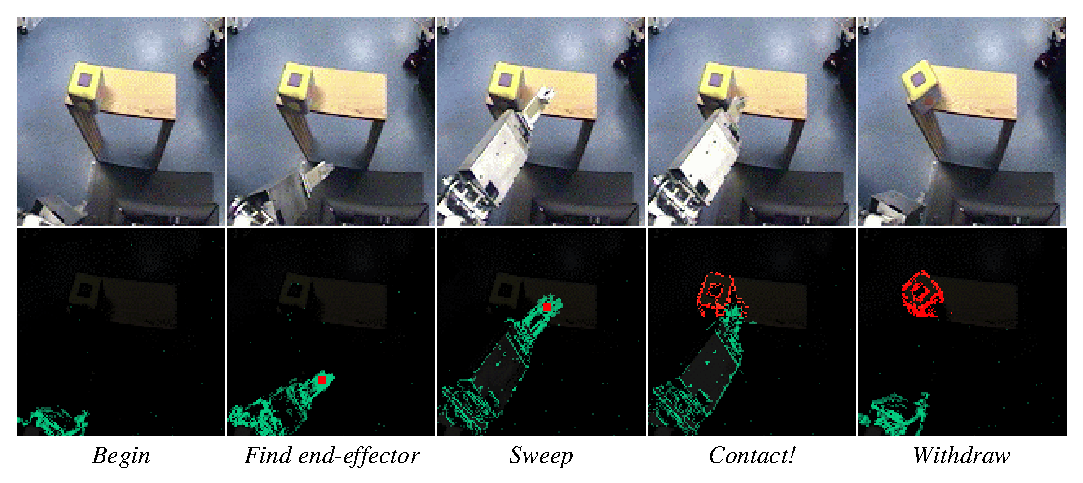
\includegraphics[width=\columnwidth]{poking-sequence.eps}

%%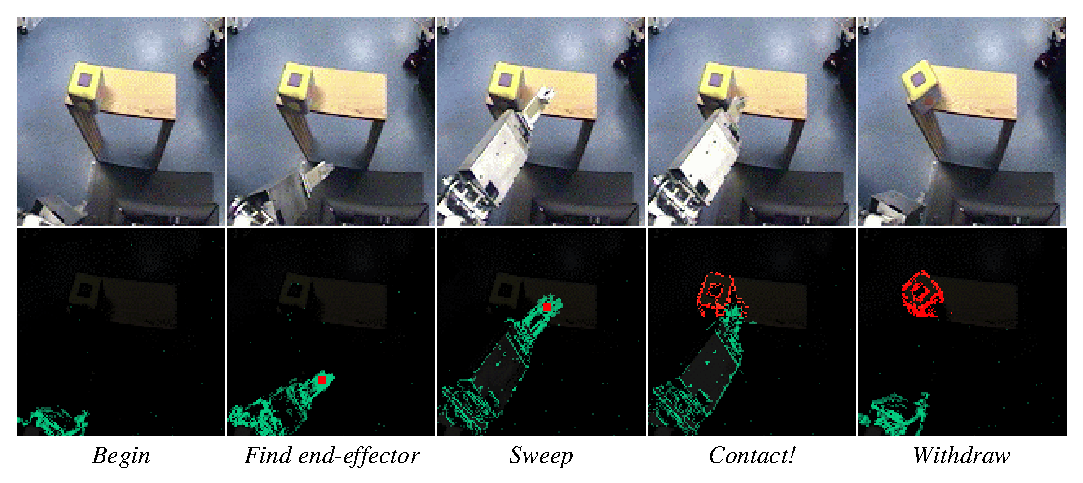
\includegraphics[width=\textwidth]{poking-sequence.eps}
%%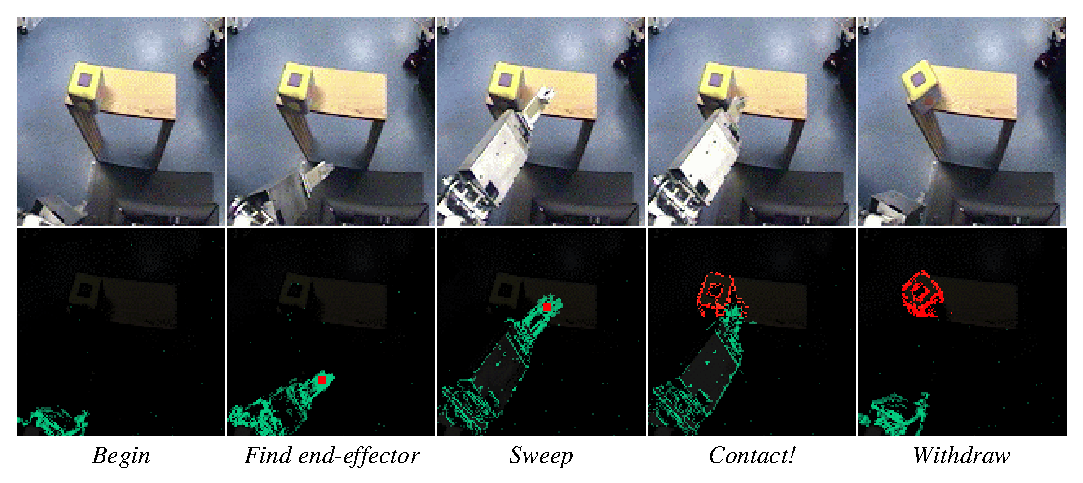
\includegraphics[width=14cm]{poking-sequence.eps}
\caption{ 
\label{fig:poking-sequence}
%
  The upper sequence shows an arm extending into a workspace, tapping
  an object, and retracting.  This is an exploratory mechanism for
  finding the boundaries of objects, and essentially requires the arm
  to collide with objects under normal operation, rather than as an
  occasional accident.  The lower sequence shows the shape
  identified from the tap using simple image differencing and flipper
  tracking.
%
}
\end{center}
\end{figure}



\section{Perceiving actions on objects}

Now that the robot knows something about its arm, it can start
to use it to explore its environment.
When the arm enters into contact with an object, one of several
outcomes are possible.  If the object is large, heavy, or otherwise
unyielding, motion of the arm may simply be resisted without any
visible effect.  Such objects are of little interest, except in their
role as obstacles, since the robot will not be able to manipulate
them.  But if the object is smaller, it is likely to move somewhat in
response to the nudge of the arm.  This movement will be temporally
correlated with the time of impact, and will be connected spatially to
the end-effector -- constraints that are not available in passive
scenarios~\cite{birchfield99depth}.  If the object is reasonably
rigid, and the movement has some component in parallel to the image
plane, the result is likely to be a flow field whose extent reflects
the physical boundaries of the object.  This visible response to
the robot's action can be used to refine its model of the object's
extent, which may be inaccurate.  For the example scene in
Figure~\ref{fig:setup-sequence} (a cube sitting on a table), the small
inner square on the cube's surface pattern might be selected as a
target.  The robot can certainly reach towards this target, but
grasping it would prove difficult without a correct estimate of the
object's physical extent.  In this section we show how the robot can
experimentally determine an object's extent using the same idea of
correlated motion used earlier to detect its own arm.

\subsubsection*{Making an impact}

Figure~\ref{fig:poking-sequence} shows how a ``poking'' movement can
be used to refine a target.  During this operation, the arm begins
by extending outwards from the resting position.  The end-effector (or
``flipper'') is localized as the arm sweeps rapidly outwards, using
the heuristic that it lies at the highest point of the region of optic
flow swept out by the arm in the image (the head orientation and
reaching trajectory are controlled so that this is true).  The arm is
driven outward into the neighborhood of the target which we wish to
define, stopping if an unexpected obstruction is reached.  If no
obstruction is met, the flipper makes a gentle sweep of the area
around the target.  This minimizes the opportunity for the motion of
the arm itself to cause confusion; the motion of the flipper is
bounded around the endpoint whose location we know from tracking
during the extension phase, and can be subtracted easily.  Flow not
connected to the end-effector can be ignored as a distractor.


The sequence shown in Figure~\ref{fig:poking-sequence} is about the
simplest case possible for segmenting the motion of the object, since most of the arm is stationary
when contact occurs.  In practice, we would rather have less
constraints on the motion of the arm, so we can approach the object
from any convenient direction.  We found that it was possible 
to attain this flexibility without losing the simplicity of object
segmentation that poking brings, by exploiting the unique
visual opportunity afforded by the moment of impact.


\ifverbose
For simplicity, the head is kept steady throughout the poking
operation, so that simple image differencing can be used to detect
motion at a higher resolution than optic flow.  Because a poking
operation currently always starts from the same location, the arm
is localized using a simple heuristic rather than the procedure described
in the previous section -- the first region of optic flow appearing
in the lower part of the robot's view when the reach begins
is assumed to be the arm.
\fi

\ifverbose
\begin{figure}[tbh]
\begin{center}
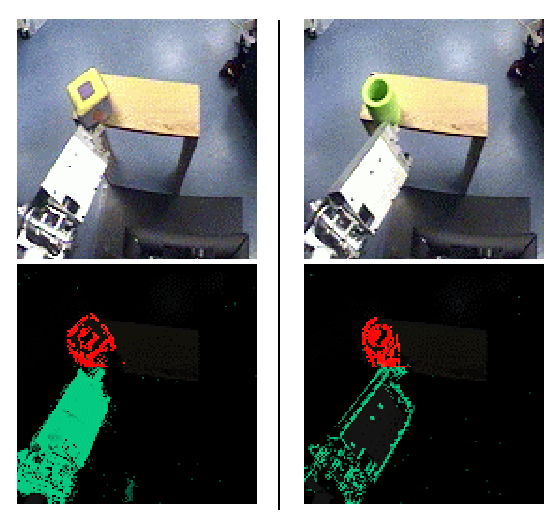
\includegraphics[width=\columnwidth]{cube-and-cylinder.eps}
\caption{ 
\label{fig:cube-and-cylinder}
%
  Poking can reveal a diffence in the shape of two objects without
  any prior knowledge of their appearance.
%
}
\end{center}
\end{figure}
\fi



\section{Detecting the point of collision}

Two components -- detecting the moment of impact, and extracting as 
much data as possible from the frames around it.

There are particular periods when the robot is attentive and fixating.
When this is so, it can detect visually when a collision occurs
between a moving object and a previously stationary object in view.
The principal task, then, is keep the motion of the moving object distinct
from that of the impacted object.

Brief introduction to image differencing and background subtraction.
Stationary camera assumption to facilitate pixel modeling.  Don't want
to keep head stationary, but can fixate for significant periods.

Image differencing is a very simple technique for detecting motion by
simply subtracting successive frames from a camera and looking for
pixel-level differences.  A moving object that has some contrast with
the background it is moving over will generate such differences.  Of
course, pixel differences can also be generated by changes in
illumination, cast shadows, computer monitors, movement of the camera
itself, etc.  A related technique called background modeling tries to
estimate the appearance of the fixed, stationary background of a 
scene, and then subtract the current view from the reference to 
detect new foreground.  While these techniques are not ideally
suited to a moving platform like our robot, they are short periods 
during which they can be useful.  In particular, when the robot is
fixating a target, we can do this.

Within the context of the robot fixating a target, we try to detect
the moment of impact precisely, so we can apply the (relatively) slow
segmentation optimization to a narrow interval of the video input and
maintain close to real-time performance.  A moving manipulator
colliding with an object will accelerate it, if it is not too massive.
If the object is rigid, the motion of the manipulator will be transmitted 
through it.  This transmission can be detected as a spreading motion
that is not plausibly generated by the manipulator itself.

Some assumptions that may fail: object not too heavy; object at least
semi-rigid; manipulator not moving above a certain speed; manipulator
not casting shadows on the object itself.  When the robot is poking the
object itself, it can control some of this.  If the object iself is
troublesome, then we potentially diagnose this, or just ignore it.

%%We are relying on some facts about optic flow.  When an object is ...

\begin{figure}[tbh]
  \begin{center}
    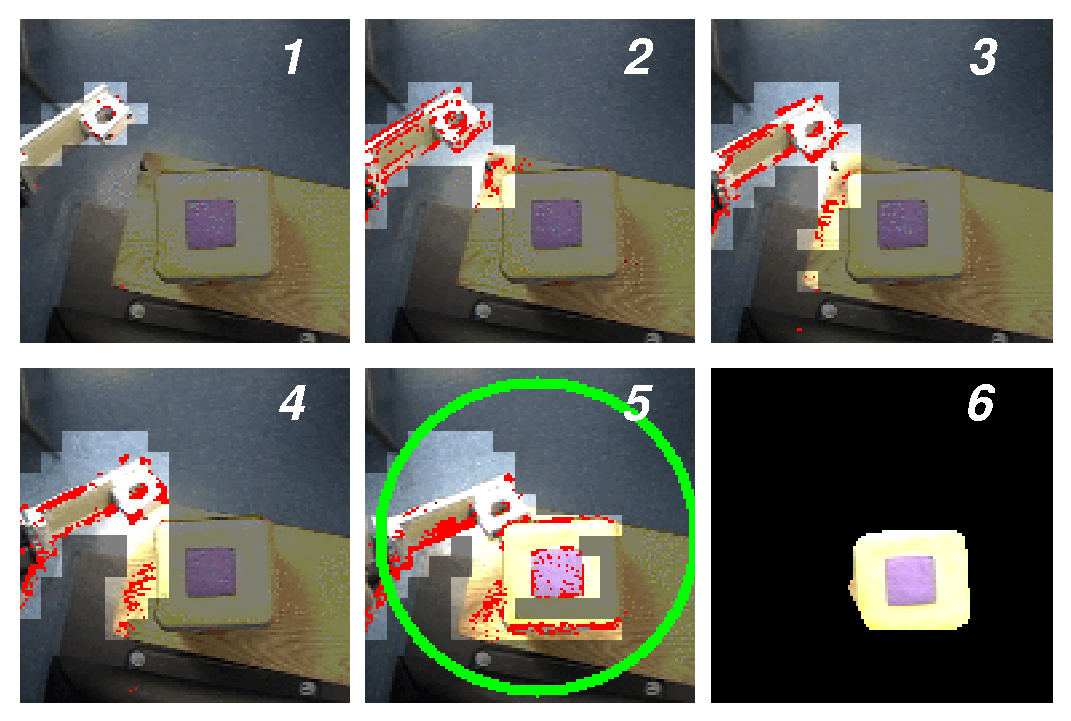
\includegraphics[width=12cm]{collision-detail}
  \end{center}
  \caption{
    The moment of impact is detected visually by the
    sudden expansion of motion away from the arm.  Motion before and
    after contact is compared to gather information for segmentation.
}
\end{figure}



\subsubsection*{An operational definition of objecthood}

The poking operation gives clear results for a rigid object that is
free to move.  What happens for non-rigid objects and objects that are
attached to other objects?  Here the results of poking are likely to
be more complicated to interpret -- but in a sense this is a good
sign, since it is in just such cases that the idea of an object
becomes less well-defined.  Poking has the potential to offer an
operational theory of ``objecthood'' that is more tractable than a
vision-only approach might give, and which cleaves better to the true
nature of physical assemblages.  The idea of a physical object is
rarely completely coherent, since it depends on where you draw its
boundary and that may well be task-dependent.  Poking allows us to
determine the boundary around a mass that moves together when
disturbed, which is exactly what we need to know for manipulation.  As
an operational definition of object, this has the attractive property
of breaking down into ambiguity in the right circumstances~-- such as
for large interconnected messes, floppy formless ones, liquids, and so
on.  Poking also gives the robot the opportunity
to collect many views of a single object, and so we can hope to deal
with recognizing objects like the cube shown in
Figure~\ref{fig:sample-results}, which look different from every side.


\begin{figure}[tbh]
  \centerline{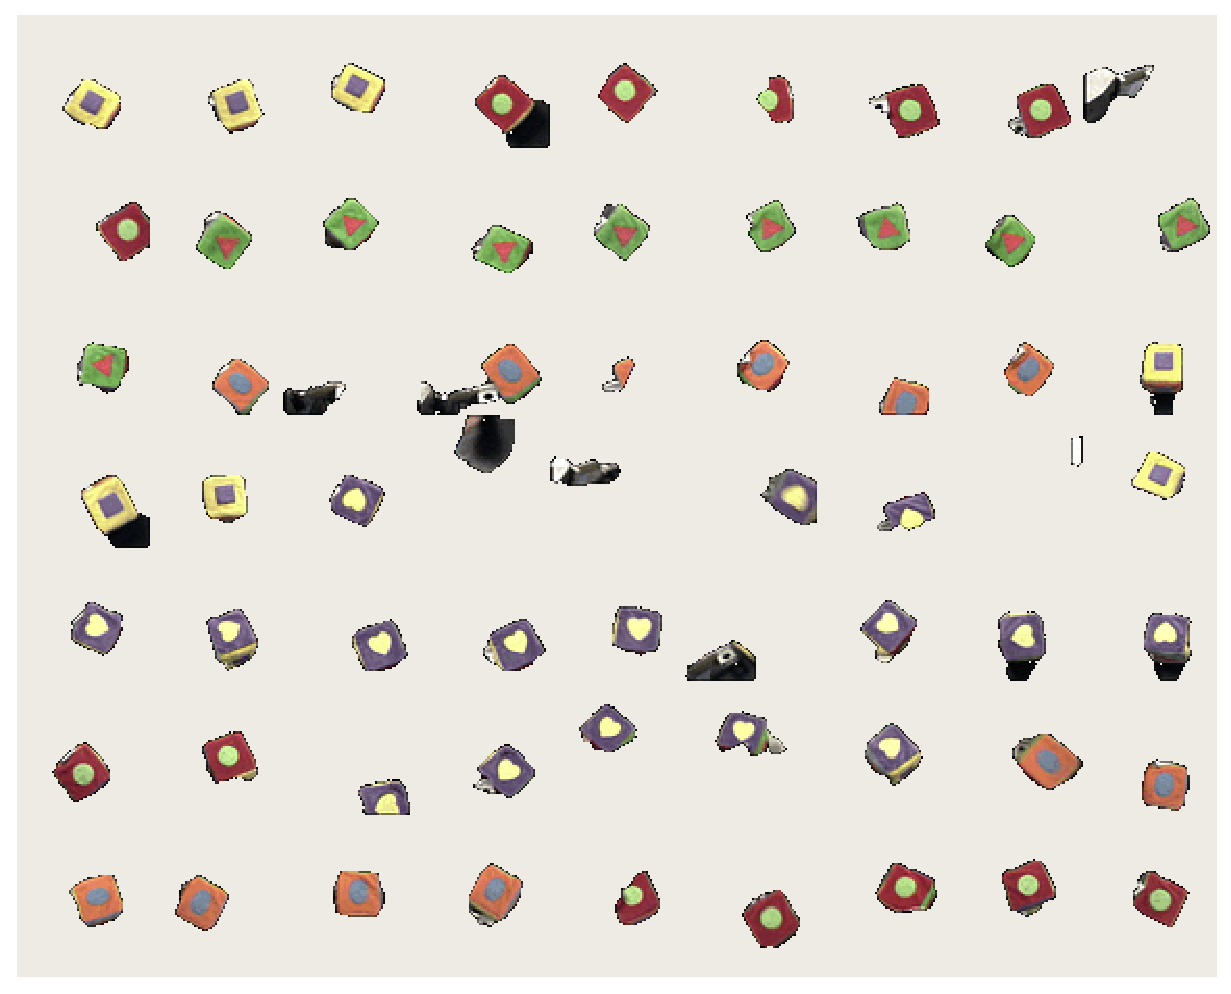
\includegraphics[width=9cm]{experiment-montage}}
  \caption{ 
  \label{fig:sample-results}
Results of a training session, where a toy cube was
  repeatedly offered to the robot for poking.  Each image of the cube
  corresponds to the segmentation found for it during a single poke.
  The most common failure mode is inclusion of the robot arm in the
  segmentation.  
}
\end{figure}



%%\clearpage \newpage



\section{Segmentation on a wearable}

Cite research abstract \citep{kemp02humans}.

Wearable computing systems have the potential to measure a great deal
of the sensory input and physical output of a person as he or she
experiences everyday activities. Much can be learned through passive
observation of these measurements. However, if we can also find ways
for the wearable system to control the behavior of the person wearing
the system, many learning tasks can be made easier.

We are designing a wearable creature that exploits a cooperative human
for its own learning purposes. Essentially, the human wearing the
system becomes the host for a parasitic creature that wishes to learn
about the world by watching and sometimes controlling the more
experienced host as he or she goes through common human activities in
the day. By using the same sensory input as the host and co-opting the
output behaviors of the host, the wearable creature serves as a top
layer of control in a subsumption architecture In essence, by
controlling the human in an effort to learn the wearable creature
changes the human into a humanoid robot.

As an initial exploration into this class of wearable applications, we
are creating a wearable system that attempts to learn common-sense
about everyday actions as they relate to objects and changes to the
environment. As shown in the figure at the top of the page, the system
currently consists of a glasses-mounted camera from which the creature
watches the world and 3 Intersense devices, each of which provides an
absolute orientation, with which the creature measures the kinematic
configuration of the host's dominant arm. The creature will also serve
as a high level controller that attempts to co-opt the host's
behaviors by requesting actions through headphones. For example, the
creature might request that its host repeat an action by uttering,
``do that again!'', which with a cooperative host should help the
creature segment the activity into meaningful parts. Likewise the
creature might ask to see an object of interest better, thereby
influencing the person to inspect the object more closely. More
generally, by requesting actions the wearable creature can test
hypotheses it has made about actions and their effect in the world.

We hope to develop a viable system for the acquisition of commonsense
related to everyday human activities. A successful creature would be
able to learn and control a set of common behaviors performed by a
cooperative human and would be able to relate common action patterns
to the visual appearance of objects and to observed changes in the
world.

\begin{figure}[bt]
\includegraphics[width=\columnwidth]{cckemp02_2}
\caption
{
cckemp 1
}
\label{fig:cckemp1}
\end{figure}


%%\clearpage \newpage

\section{Segmentation through periodicity}

Cite research abstract~\citep{arsenio02boosting}.

\subsection{Waving the object}

\subsection{Waving the hand/arm/finger}

Through direct embodied actuation

  Teacher waves objects to the robot

Human arm/hand/finger waving for segmentation

Robust: to humans, other objects moving in the background --
ignored if they are non-periodic

Powerful technique for segmenting stationary objects e.g. Objects
painted in a book

Heavy, stationary objects: table, sofa

Using relative size of the arm, can get relative size of objects

Through indirect embodied actuation

 Teacher waves arm/hand/finger to create a pop-out effect
       finger trajectory groups segmented regions together

Method:

1)  Detect Motion > Th

     Detect Skin tones for arm/hand/finger  > Th

2) Initialize grid of points in moving region

3) Track these points over the window interval (32 and 64 frames)

     - using optical flow

4) Compute WFFTs for the temporal signal of each point

5) Select signals with a single peak of energy over all frequencies 


\begin{figure}[bt]
\includegraphics[width=\columnwidth]{fig-artur1}
\caption
{
artur 1
}
\label{fig:artur1}
\end{figure}

%%\newpage

\begin{figure}[bt]
\includegraphics[width=\columnwidth]{fig-artur2}
\caption
{
artur 2
}
\label{fig:artur2}
\end{figure}


%%\clearpage \newpage
